%% FEUP THESIS STYLE for LaTeX2e
%% how to use feupteses (English version)
%%
%% FEUP, JCL & JCF, 31 July 2012
%%
%% PLEASE send improvements to jlopes at fe.up.pt and to jcf at fe.up.pt
%%

%%========================================
%% Commands: pdflatex tese
%%           bibtex tese
%%           makeindex tese (only if creating an index)
%%           pdflatex tese
%% Alternative:
%%          latexmk -pdf tese.tex
%%========================================

\documentclass[11pt,a4paper,twoside,openright]{report}

%% For iso-8859-1 (latin1), comment next line and uncomment the second line
\usepackage[utf8]{inputenc}
%\usepackage[latin1]{inputenc}

%% English version

%% MIEIC options
\usepackage[mieic]{feupteses}
%\usepackage[mieic,juri]{feupteses}
%\usepackage[mieic,final]{feupteses}
%\usepackage[mieic,final,onpaper]{feupteses}

% For gantt timeline diagrams
\usepackage{pgfgantt}

%% Additional options for feupteses.sty: 
%% - onpaper: links are not shown (for paper versions)
%% - backrefs: include back references from bibliography to citation place

%% Uncomment the next lines if side by side graphics used
%\usepackage[lofdepth,lotdepth]{subfig}
%\usepackage{graphicx}
%\usepackage{float}

%% Include color package
\usepackage{color}
\definecolor{cloudwhite}{cmyk}{0,0,0,0.025}

%% Include source-code listings package
\usepackage{listings}
\lstset{ %
 language=C,                        % choose the language of the code
 basicstyle=\footnotesize\ttfamily,
 keywordstyle=\bfseries,
 numbers=left,                      % where to put the line-numbers
 numberstyle=\scriptsize\texttt,    % the size of the fonts that are used for the line-numbers
 stepnumber=1,                      % the step between two line-numbers. If it's 1 each line will be numbered
 numbersep=8pt,                     % how far the line-numbers are from the code
 frame=tb,
 float=htb,
 aboveskip=8mm,
 belowskip=4mm,
 backgroundcolor=\color{cloudwhite},
 showspaces=false,                  % show spaces adding particular underscores
 showstringspaces=false,            % underline spaces within strings
 showtabs=false,                    % show tabs within strings adding particular underscores
 tabsize=2,                     % sets default tabsize to 2 spaces
 captionpos=b,                      % sets the caption-position to bottom
 breaklines=true,                   % sets automatic line breaking
 breakatwhitespace=false,           % sets if automatic breaks should only happen at whitespace
 escapeinside={\%*}{*)},            % if you want to add a comment within your code
 morekeywords={*,var,template,new}  % if you want to add more keywords to the set
}

%% Uncomment to create an index (at the end of the document)
%\makeindex

%% Path to the figures directory
%% TIP: use folder ``figures'' to keep all your figures
\graphicspath{{figures/}}

%%----------------------------------------
%% TIP: if you want to define more macros, use an external file to keep them
%some macro definitions

% format
\newcommand{\class}[1]{{\normalfont\slshape #1\/}}

% entities
\newcommand{\Feup}{Faculdade de Engenharia da Universidade do Porto}

\newcommand{\svg}{\class{SVG}}
\newcommand{\scada}{\class{SCADA}}
\newcommand{\scadadms}{\class{SCADA/DMS}}

%%----------------------------------------

%%========================================
%% Start of document
%%========================================
\begin{document}

%%----------------------------------------
%% Information about the work
%%----------------------------------------
\title{From simulation to development in MAS: Repast-JADE automatic code generation for interaction protocols}
\author{João Pedro Camacho Lopes}

%% Uncomment next line for date of submission
%\thesisdate{July 31, 2008}

%%Uncomment next line for copyright text if used
%\copyrightnotice{Name of the Author, 2008}

\supervisor{Supervisor}{Henrique Lopes Cardoso}

%% Uncomment next line if necessary
%\supervisor{Second Supervisor}{Name of the Supervisor}

%% Uncomment committee stuff in the final version if used
%\committeetext{Approved in oral examination by the committee:}
%\committeemember{Chair}{Doctor Name of the President}
%\committeemember{External Examiner}{Doctor Name of the Examiner}
%\committeemember{Supervisor}{Doctor Name of the Supervisor}
%\signature

%% Specify cover logo (in folder ``figures'')
\logo{uporto-feup.pdf}

%% Uncomment next line for additional text  below the author's name (front page)
%\additionalfronttext{VERSÃO PRELIMINAR PDIS}

%%----------------------------------------
%% Preliminary materials
%%----------------------------------------

% remove unnecssary \include{} commands
\begin{Prolog}
  %!TEX root = thesis.tex
\chapter*{Abstract}

%Multi-agent systems (MAS) present an interesting approach to the efficient development of modular systems. MAS are composed by autonomous computational units called agents that are programmed to \emph{compete} or \emph{work together}, for instance in order to solve computational problems, engage in automatic negotiation or play computer games. Frameworks exist that aid the development of this class of systems and they range from mostly general-purpose frameworks to domain-specific in an array of different domains.
%
%Multi-agent-based simulations (MABS) are sometimes used on the course of development of a full-featured MAS - for instance, for testing purposes. However, most platforms for MAS development are not well suited for MABS development \cite{mengistu2008scalability}.
%
%JADE \cite{bellifemine2003jade}, a very popular MAS development framework allows the creation of seamless distributed agent systems and complies with FIPA standards for agent interaction. Unfortunately, its multi-threaded architecture falls short in delivering the necessary performance to run a local simulation with a large number of agents. Repast \cite{collier2003repast} is an agent-based simulation toolkit that allows creating simulations using rich GUI elements and real time agent statistics. Unlike JADE, though, Repast lacks much of the infrastructure for agent creation and interaction.
%
%Some authors \cite{garcia2011misia,gormer2011jrep}, as reviewed in this report, proposed an integration of JADE and Repast by means of a middleware, essentially representing the agent in both and taking advantage of the features provided by the frameworks.
%
%In this thesis, a code generation tool is proposed, capable of not only generating a Repast simulation from an existing JADE MAS, but also of creating a full featured JADE application from a Repast-based simulation. An implementation of FIPA's interaction protocols will be proposed for Repast as a means to deliver the mentioned conversion tool. The most immediate advantage over the previous approaches is that existing systems can make use of this tool to create appropriate simulations where agent interaction can be more easily analyzed. Furthermore, proficient programmers in one framework can quickly get started in the development for the complementary framework.


\chapter*{Resumo}
%
%Os sistemas multi-agente (SMA) exprimem uma abordagem interessante no desenvolvimento de sistemas modulares e eficientes. Os MAS são compostos por elementos computacionais autónomos - chamados agentes - que são programados para \emph{competir} ou \emph{colaborar} de modo a, por exemplo, resolver problemas computacionais, iniciar negociação automática ou participar em jogos de computador. Existem ferramentas de software que facilitam o desenvolvimento desta classe de sistemas que podem variar entre ferramentas de âmbito geral até ferramentas focadas num domínio específico.
%
%As simulações baseadas em agente (SBA) são frequentemente utilizadas durante o desenvolvimento de MAS completos - por exemplo, afim de testar o sistema. No entanto, a maior parte das plataformas para desenvolvimento de SMA não são apropriadas para a criação de SBA \cite{mengistu2008scalability}.
%
%O JADE \cite{bellifemine2003jade} é um exemplo de uma plataforma de desenvolvimento de SMA que permite a criação de sistemas distribuídos de agentes de forma simplificada cumprindo, ainda, os standards da FIPA (\emph{Foundation for Intelligent Physical Agents}) sobre protocolos de interação entre agentes. No entanto, a sua arquitetura em \emph{multi-thread} não garante a performance necessária para a execução de simulações com um elevado número de agentes. O Repast \cite{collier2003repast} é uma plataforma de criação de simulações baseadas em agentes que permite criar simulações ricas em interfaces gráficas para visualização de dados históricos e em tempo real sobre os agentes. Ao contrário do JADE, o Repast não dispõe de uma infraestrutura para criação de agentes e interação entre eles.
%
%Alguns autores estudados neste relatório \cite{garcia2011misia,gormer2011jrep} propõem uma integração entre o JADE e o Repast por meio de uma camada de software intermédio, fazendo representar cada agente duplamente - uma vez em cada plataforma, essencialmente tirando partido das capacidades de ambas as plataformas em simultâneo.
%
%Para esta dissertação é proposta uma ferramenta de geração automática de código capaz não só de gerar uma simulação baseada em Repast a partir de um SMA baseado em JADE, mas também de criar um SMA em JADE partindo de uma simulação baseada em Repast. Será também criada uma proposta de implementação, para a plataforma Repast, dos standards da de interação entre agentes da FIPA, tornando possível a conversão de código entre as duas plataformas. A vantagem mais imediata sobre a proposta anterior é que SMA já existentes podem tirar partido da ferramenta proposta para rapidamente criar uma simulação com funcionamento equivalente e ter acesso a ferramentas de visualização e estatísticas do sobre o comportamento dos agentes. Adicionalmente, programadores proficientes numa das plataformas pode iniciar rapidamente o desenvolvimento da plataforma complementar. % the abstract
  % \chapter*{Acknowledgements}

Aliquam id dui. Nulla facilisi. Nullam ligula nunc, viverra a, iaculis
at, faucibus quis, sapien. Cum sociis natoque penatibus et magnis dis
parturient montes, nascetur ridiculus mus. Curabitur magna ligula,
ornare luctus, aliquam non, aliquet at, tortor. Donec iaculis nulla
sed eros. Sed felis. Nam lobortis libero. Pellentesque
odio. Suspendisse potenti. Morbi imperdiet rhoncus magna. Morbi
vestibulum interdum turpis. Pellentesque varius. Morbi nulla urna,
euismod in, molestie ac, placerat in, orci. 

Ut convallis. Suspendisse luctus pharetra sem. Sed sit amet mi in diam
luctus suscipit. Nulla facilisi. Integer commodo, turpis et semper
auctor, nisl ligula vestibulum erat, sed tempor lacus nibh at
turpis. Quisque vestibulum pulvinar justo. Class aptent taciti
sociosqu ad litora torquent per conubia nostra, per inceptos
himenaeos. Nam sed tellus vel tortor hendrerit pulvinar. Phasellus
eleifend, augue at mattis tincidunt, lorem lorem sodales arcu, id
volutpat risus est id neque. Phasellus egestas ante. Nam porttitor
justo sit amet urna. Suspendisse ligula nunc, mollis ac, elementum
non, venenatis ut, mauris. Mauris augue risus, tempus scelerisque,
rutrum quis, hendrerit at, nunc. Nulla posuere porta orci. Nulla dui. 

Fusce gravida placerat sem. Aenean ipsum diam, pharetra vitae, ornare
et, semper sit amet, nibh. Nam id tellus. Etiam ultrices. Praesent
gravida. Aliquam nec sapien. Morbi sagittis vulputate dolor. Donec
sapien lorem, laoreet egestas, pellentesque euismod, porta at,
sapien. Integer vitae lacus id dui convallis blandit. Mauris non
sem. Integer in velit eget lorem scelerisque vehicula. Etiam tincidunt
turpis ac nunc. Pellentesque a justo. Mauris faucibus quam id
eros. Cras pharetra. Fusce rutrum vulputate lorem. Cras pretium magna
in nisl. Integer ornare dui non pede. 

\vspace{10mm}
\flushleft{The Name of the Author}
  % the acknowledgments
  % \cleardoublepage
\thispagestyle{plain}

\vspace*{8cm}

\begin{flushright}
   \textsl{``You should be glad that bridge fell down. \\
           I was planning to build thirteen more to that same design''} \\
\vspace*{1.5cm}
           Isambard Kingdom Brunel
\end{flushright}
       % initial quotation if desired
  \cleardoublepage
  \pdfbookmark[0]{Table of Contents}{contents}
  \tableofcontents
  \cleardoublepage
  \pdfbookmark[0]{List of Figures}{figures}
  \listoffigures
  \cleardoublepage
  \pdfbookmark[0]{List of Tables}{tables}
  \listoftables
  %!TEX root = thesis.tex
\chapter*{Abbreviations}
\chaptermark{ABBREVIATIONS}

\begin{flushleft}
\begin{tabular}{l p{0.8\linewidth}}
ACL		 & Agent Communication Language \\
AST		 & Abstract Syntax Tree \\
ATL		 & ATLAS Transformation Language \\
CeCILL-C	& CEA CNRS INRIA Logiciel Libre (open source license) \\
EPL		 & Eclipse Public License (open source license) \\
FIPA	 & Foundation for Intelligent Physical Agents \\
FOSS 	 & Free and Open Source Software \\
IDE 	 & Integrated Development Environment \\
JADE	 & Java Agent DEvelopment Framework \\
JDT		 & [Eclipse] Java Development Tools \\
MABS	 & Multi-Agent-Based Simulation \\
MAS      & Multi-Agent System \\

\end{tabular}
\end{flushleft}

  % the list of abbreviations used
\end{Prolog}

%%----------------------------------------
%% Body
%%----------------------------------------
\StartBody

%% TIP: use a separate file for each chapter
%!TEX root = thesis.tex
\chapter{Introduction}
\label{chap:intro}

\section*{}

Multi-agent systems (MAS) are composed of autonomous computational elements capable of interacting with each other, called agents. The development of this class of systems comprise an interesting software paradigm but in terms of computer science history, MAS are a recent subject, having gained significant traction only after the mid 1990's \cite{wooldridge2008introduction}. With multiple applications such as problem solving, simulation, trading, negotiation, computer games and logistics using an efficient and modular development approach, MAS enjoyed a rapid growth in popularity and are in widespread use nowadays \cite{ferber1999multi}.

\section{Context}

Although their use is certainly widespread, there is no single general purpose standard for MAS development, since each system has different needs. Many times, such systems are created from scratch, meaning that the developers must define all features of the system - such as its agents, their behavior, communication and organization, using conventional programming languages and tools. However, several frameworks exist that offer some level of abstraction from the code, allowing for a more conceptual approach to
MAS development \cite{gormer2011jrep}. 

Most uses of MAS, for instance in negotiation, games or logistics, demand a small number of agents, typically with larger resource demands but also without any need for control global control of execution, i.e. it is perfectly reasonable for these types of systems to be based on events and for its agents to work asynchronously. In contrast, multi-agent-based simulations (MABS) are usually implemented using a large number of lightweight agents with a small resource footprint. MAS development frameworks generally provide the programmer with a range of features such as execution control, communication protocols or agent awareness capabilities. In spite of that, most frameworks that focus on MAS development lack synchronization mechanisms and lightweight agent infrastructure required by MABS. One of the main goals of simulations is to be able to visualize real-time, as well as historical data that allow to study emergent and evolutionary phenomena. \cite{mengistu2008scalability}


\section{Motivation} \label{sec:goals}


The motivation for this thesis pertains the study of the development of agent-based software, focusing on the notion that MAS and MABS can both integrate the same project. As said before, MAS and MABS developers expect different groups of features to be provided by the development frameworks. Furthermore, in the course of development, a need may arise to use a different set of features. For instance, while developing a large scale MAS, a need for creating a simulation based on the same model may arise. The reverse can occur as well - the development may start as a simulation that later must be implemented with another kind of framework.

This thesis will focus on using two frameworks that are very popular in their respective domain. First we have JADE, a framework that attempts to simplify the development of distributed agent application by seamlessly hiding all complexity concerning its distributed architecture. JADE is also FIPA compliant, meaning that is much easier to create an open MAS. With JADE, the programmers ``can focus their software development just on the logic of the application rather than on middleware issues, such as discovering and contacting the entities of the system'' \cite{bellifemine2003jade}. The second selected framework was Repast, a toolkit that provides objects for the creation and execution of MABS, while allowing the programmer to collect data from the agents. With Repast it is also fairly simple to create a wide range of different charts to represent the collected data.

\begin{table}[tb]
	\caption{Summary of JADE and Repast features.}
	\label{tab:jadevsrep}
	\begin{center}
		\begin{tabular}{l|ccc}
		\hline

		\hline
		\textbf{} & \textbf{JADE} & \textbf{Repast} & \textbf{Cougaar} \\
		\hline
			Communication & FIPA ACL &  Method calls  & Serialized Object \\
						  &			 &  Shared resources \\
		\hline
			Distribution & Yes & No & Yes \\
		\hline
			Simulation Tools & No & Yes & Yes \\
		\hline
			Scalability & Limited & High & High \\
		\hline
			Ontologies & Yes & No & Yes\\
		\hline
			Open Source & Yes & Yes & Yes\\
		\hline
			Agent Execution & Behavior-based & Schedule-based  &  \\
							& Multi-threaded & Single-threaded &  \\
							& Event-driven   & Tick-driven 	   &  \\
							& Assync		 & Sync 		   &  \\
		\hline
		\end{tabular}
	\end{center}
\end{table}

While JADE excels in creating seamless, distributed, peer-to-peer systems,
Repast's strength is in creating simulations as well as collecting and displaying statistical data in different ways. In JADE, as table \ref{tab:jadevsrep} illustrates, agents execute in separate threads and while this architecture facilitates the platform's distribution, JADE's agent are heavy in terms of resources. Experiments with JADE show that the platform's scalability is limited in number of agents and that the global system performance drops quickly for large number of agents \cite{mengistu2008scalability} \cite{garcia2011misia}.

JADE and Repast were chosen over other platforms mainly for their popularity and widespread use - not dismissing their quality, of course. As an example of an alternative framework, Cougaar (Cognitive Agent Architecture) solves the problem explain above by proposing a fully featured agent architecture, while maintaining high performance and scalability required for simulation. It doesn't, however, implement any interaction standards; messages are exchanged by means of serialized Java objects \cite{helsinger2004cougaar}. Table \ref{tab:jadevsrep} presents a rundown of the comparison of these frameworks.

The analysis made in this section applies to JADE version 4.3.1 (6 December 2013) and Repast Symphony 2.1 (12 August 2013), which are also the versions that will be used throughout the production of this thesis.


\section{Goals}
The first goal of this thesis is to create a code conversion tool. This tool enables the programmer to generate a Repast simulation automatically from the source code of a JADE application (development to simulation), as well as obtaining a proper multi agent system in JADE starting from a Repast simulation (simulation to development). Such a conversion tool not only allows the developer to quickly deploy a MAS or create a simulation, as explained before, but also enables a proficient programmer in one framework to quickly get started in developing with the other framework.

The second goal is to bring communication standards to Repast. While JADE complies with the FIPA standards for agent interaction, Repast implements no standards at all. Creating a library for implementation of FIPA interaction protocols in Repast will not only enrich that framework but will make the code generation more straightforward.

One of the soft goals for the final product is that the programmer should not be forced to introduce significant changes to the original code in order to be able to use the tool. The generated code must also preserve the functionality of the original code - meaning that the re-conversion must generate code that is equivalent to the original one.

It's important to note that the main focus of this thesis is to convert agent interaction between the two frameworks. Agent behavior can be far more complex and go beyond simply agent interaction and, while the initial work will be laid down to allow for future work on perfectly mimicking agent behavior, this is not a main goal.
 

\section{Thesis contents} \label{sec:struct}

To summarize, this report proposes the development of a tool that converts a MABS created in Repast into MAS that uses JADE. Conversely, it should allow the conversion of a JADE MAS into a Repast MABS as well. This tool is useful in the context of development of a MAS that either started as a MABS or when the need to create a simulation arises during development. JADE and Repast were chosen for this thesis not only for their quality but also for their widespread use.

After this introduction, chapter \ref{chap:sota} starts by discussing some related work about JADE, Repast and about integrating both frameworks. A great part of this thesis will be about Java code transformations, since the goal is to convert the code from one framework to the other. Therefore, part of the state-of-the-art review was related to code transformation tools.

Chapter \ref{chap:validation} describes the details of the development environment as well as the definition of how the final product will be validated and evaluated. Chapter \ref{chap:plan} includes a detailed work plan for the following months and finally, \ref{chap:concl} includes final notes about this report and about the work done so far. 
%!TEX root = thesis.tex
\chapter{Bibilography Review} \label{chap:sota}

\section*{}

% Neste capítulo é descrito o estado da arte e são apresentados trabalhos
% relacionados para mostrar o que existe no mesmo domínio e quais os problemas
% em aberto. Deve deixar claro que existe uma oportunidade de desenvolvimento
% que cobre alguma falha concreta .

% O capítulo deve também efetuar uma revisão tecnológica às principais
% ferramentas utilizáveis no âmbito do projeto, justificando futuras escolhas.

This chapter presents a summary and analysis of some works related to the use of Repast and JADE frameworks in the development of MAS. The related
work is sorted in four categories.

The first category includes a discussion about existing works on integrating both JADE and Repast simultaneously by developing a middleware framework.  While the goal of this thesis is not to use both frameworks simultaneously, these works give a valuable insight into the shortcomings of both frameworks as well as providing some interesting comparisons between their features. The second category includes discussion about implementations of these protocols in Repast. Then, the third category presents some existing Java code generation and transformation tools. These tools will give support to the automation of code refactoring, detection of code patterns and library calls. This chapter ends with a summary of the bibliography review and an overview of the most interesting topics approached in this chapter.

\section{JADE and Repast integration}
JADE is a very popular framework for developing MAS, providing an infrastructure that allows the programmer to create a distributed system in a very transparent way. As discussed before, in the motivation for this thesis, JADE is not the best tool to develop a MABS, not only because it lacks the visualization tools that other frameworks provide for displaying data about agent behavior, but also because due to its multi threaded architecture JADE has performance issues when the system comprises a large number of agents. Following are two frameworks created to bridge these two worlds of MAS development and simulation by integrating Repast and JADE in the same platform by means of a middleware.

\subsection{MISIA: Middleware Infrastructure to Simulate Intelligent Agents}

	MISIA is a middleware whose goal is to enhance the simulation of intelligent agents and to allow the visualization and analysis of agent's behavior. Not only does MISIA allow ``simulation, visualization and analysis of the agent’s behavior'', but also ``makes use of technologies for the development of multi-agent systems known and widely used, and combines them so that it is possible to use their capabilities to build highly complex and dynamic systems.'' In Garcia \textit{et al}, the authors chose to develop this framework on top of JADE and Repast Symphony. Their reasoning lies on the widespread use of JADE as an agent-based software development middleware, on Repast being simple and well documented and finally on both frameworks being open source. \cite{garcia2011misia}


	Most platforms like JADE lack organizational features and support for simulation constraints - this infrastructure must be developed by the programmer. The main concept introduced to JADE by MISIA is the concept of time - synchronization is fundamental for simulation. MISIA also brings the possibility to develop open MAS in Repast by taking advantage of JADE implementation of FIPA protocols.

	\begin{figure}[h]
	  \begin{center}
	    \leavevmode
	    \includegraphics[width=.7\textwidth]{misia}
	    \caption{Functional structure of MISIA \cite{garcia2011misia}}
	    \label{fig:misiadiagram}
	  \end{center}
	\end{figure}

	As illustrated in the diagram on figure \ref{fig:misiadiagram}, MISIA consists of three layers of components: a layer of contact with Repast; an intermediate layer between the two frameworks; a layer that interfaces with JADE and enables the concept of time in that framework.

	The purpose of the `JADE layer' is for JADE's agents to perform their actions in each tick - the smallest unit of time in a Repast-based simulation. The synchronization of JADE's agents is made by informing them about the current tick. MISIA uses an agent for this - dubbed `synchronizer' - that acts as a notifier. Furthermore, FIPA protocols are implemented with a wrapper that adapts them to Repast ticks.

	Besides creating a wrapper on JADE's agents and FIPA protocols, an extra agent was included in the Repast layer. This means that for each agent created with MISIA, there are actually two agents being created. This layer also lets the synchronizer know that a new tick has passed.

\subsection{JREP - Extending Repast Symphony for JADE Agent Behavior Components}
	In Gömer \textit{et al} \cite{gormer2011jrep}, the authors propose JREP, another platform for integrating JADE and Repast Symphony in the same framework, by means of a middleware. To demonstrate its use, the authors present an example of a smart airport and how it can be simulated using JREP.

\begin{quote}
	``JREP [is] a novel integration of JADE and Repast Symphony that efficiently combines the macro and micro perspective with an interaction layer. It allows to see not only the overall system behavior, but also the individual together with its interests, goals and the communication to
	others for local coordination and cooperation. Scheduling of the agents, (time) synchronization and the registration of new agents with the environment has been solved.'' \cite{gormer2011jrep}
\end{quote}

	The rationale for their choosing of JADE and Repast Symphony as working platforms is well defined:
	Repast provides statistical functions, real-time monitoring, graphs and history recording; it also supports external statistical programs and has good execution speed.
	JADE, on the other hand, is pointed as having a highly efficient message transport layer. 

	JREP's architecture is similar to that of MISIA. There are three layers where the first one, called \textit{macro level} interacts with Repast, providing the scheduling mechanism; the second one, which they called \textit{micro level}, interacts with JADE and contains the behavior objects and the third one, called \textit{interaction level} which handles agent interaction using FIPA ACL.
	Agents in JREP are represented as both a Repast Agent and a JADE Agent. The main difference to MISIA is that in JREP the Repast Agent contains the reference to the respective JADE agent while is MISIA this was handled by an intermediate layer.

\subsection{Similar work}
	Other works related to integration of features from Repast and JADE are available. This, however, is not the main focus of this thesis since its goal is not to use both frameworks simultaneously. That said, there is some interest in these works, as I explained in the beginning of this chapter. 

% end % JADE and Repast integration

\section{FIPA standards in Repast}
	MISIA and JREP both attempted to complement Repast's lack of communication protocols by creating an interface with JADE's implementation of FIPA interaction protocols. 

	Open source projects exist that contemplate the use of FIPA ACL as a library, but none was found to be actively maintained or properly documented. Therefore, this thesis will contemplate the creation of a Java library that brings FIPA standards to Repast.
% end % FIPA standards in Repast


\section{Code generation}
	There are multiple ways to tackle the problem of code transformations, as described in this thesis. The brute force approach would be to parse the source code, create an abstract syntax tree (AST), which represents all code constructions in a program, perform certain transformations in the tree, and then generate back the code from the new AST. Fortunately, there are free and open source projects that developers can use to do exactly this with significantly reduced effort. From the available tools, I selected the ones that are the most relevant to this thesis, i.e. tools for Java code transformation that are open source, well documented and still supported. 

\subsection{Eclipse Java Development Tools (JDT)}

	The Java Development Tools are are a group of plug-ins that provide Eclipse the necessary means to become a full-featured Java IDE.
	These tools make up what we perceive as the ``Eclipse IDE'' and programmers can use these libraries in their Java projects and perform tasks that require a certain introspection of the code itself. Some of the possibilities presented by Eclipse JDT that could be interesting for this thesis are the creation of projects (in runtime and programmatically) which would allow the generated code to be shown immediately in the IDE; accessing projects in the workspace, allowing the programmer to access the project's code; finding calls to methods, very useful for mapping library calls from one framework to the other (for instance) and AST parsing, for a lower level parsing of code, allowing to directly manipulate methods and data structures \cite{eclipseJDT}.

	JDT can be broken down into five main components: 

	\begin{description}
		\item[APT] - Annotation Processing Tool\hfill \\
  			This component can be used to parse annotations in the code. Annotations are a Java construction introduced in Java 5 and can be used to add meta information about classes, objects and methods. These annotations can then be parsed by frameworks that use the POJO (plain old Java objects) that enclose them. As an example in the context of the code generation tool, annotations could be used to select entities like agents or data structures in a JADE project that would then be visualized in a Repast chart.
		\item[Core] - Java IDE headless infrastructure \hfill \\
  			The core for the Java IDE, it allows to transverse the Java element tree and find package fragments, compilation units, binary classes, types, methods and fields. This tool could be useful for mapping methods and library calls from one framework to another.
		\item[Debug] - Debug support for Java\hfill \\
  			This tool makes the debug facilities of Eclipse possible. It provides functionalities such as execution control and contextual expression evaluation. It will probably not be very useful in the context of this thesis
		\item[Text and UI] - Java editing support and Java IDE user interface \hfill \\
  			These components make development in Eclipse possible by providing a GUI for code editing, enriched with syntactic errors highlighting, among other interesting aids. This component is not immediately necessary for the development of the code generation tool.
	\end{description}


\subsection{Spoon - Program Analysis and Transformation in Java}
	Spoon is a tool created to take advantage of the new features introduced on the release of Java 5, namely annotations and generics. It is a Java transformation tool that uses annotation processing, compile-time reflection and templates in a pure-Java environment to enable programmers to create their own platforms for code transformations. As illustrated by figure \ref{fig:spoon-compile}, these transformations occur on compile time and annotations are used as parameters for compilation. The programmer uses plain Java code to define the transformations that should occur, for instance, adding code snippets to the beginning of a method in a class. Finally, Spoon can be seamlessly integrated in an IDE such as Eclipse \cite{spoon,pawlak2006spoon}.

	\begin{figure}[h]
	  \begin{center}
	    \leavevmode
	    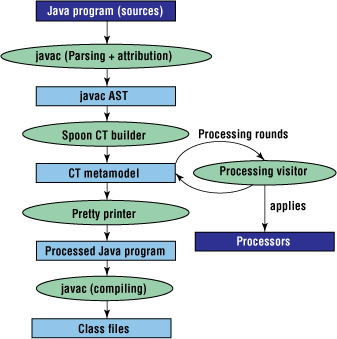
\includegraphics[width=.5\textwidth]{spoon-compile}
	    \caption{Spoon compile-time processing \cite{pawlak2006spoon}}
	    \label{fig:spoon-compile}
	  \end{center}
	\end{figure}

\subsection{ATL - ATL Transformation Language }
	ATL - \emph{ATLAS Transformation Language}, is both the name of a language and its enclosing plug-in and allows the creation of model transformations. Unlike JDT and Spoon analyzed before, ATL does not focus on applying transformations to the source code.

	\begin{figure}[h]
	  \begin{center}
	    \leavevmode
	    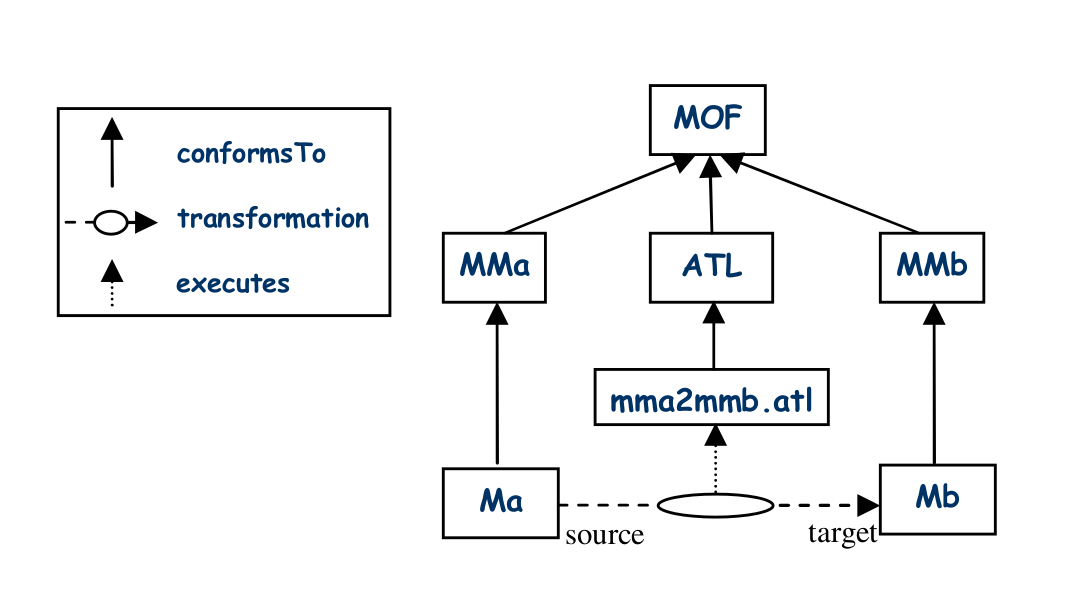
\includegraphics[width=.7\textwidth]{atl}
	    \caption{Overview of ATL transformational approach \cite{jouault2006transforming}}
	    \label{fig:so-atl-wow}
	  \end{center}
	\end{figure}

	\begin{quote}
		``ATL is applied in a transformational pattern shown in Fig. 1 . In this pattern a source model Ma is transformed into a target model Mb according to a transformation definition mma2mmb.atl written in the ATL language. The transformation definition is a model. The source and target models and the transformation definition conform to their metamodels MMa, MMb, and ATL respectively. The metamodels conform to the MOF metametamodel.''
	\end{quote}

	As explained in Jouault \emph{et al} and as illustrated in figure \ref{fig:so-atl-wow} by the same authors, ``a source model Ma is transformed into a target model Mb according to a transformation definition mma2mmb.atl written in the ATL language'', which is also a model itself. The three must conform to their respective metamodels MMa, MMb and ATL which then conform to the metametamodel MOF.
% end % Code generation tools


\section{Summary}
Although the specific problem of converting code between JADE and Repast has not been approach before in the available literature, it is clear that some related work is useful in the definition of a solution proposed in this thesis. JREP and MISIA show is that interoperability between the two frameworks is possible and helped defining the limitations of each framework. The usefulness of these works is limited, though, since the source code is not readily available and it is unknown if either project is still being developed and supported. Also, one of the goals proposed in the Introduction refers to the ability to generate code with introducing extensive changes to the original code. What JREP and MISIA propose is a platform to build new systems from the beggining using JADE and Repast.

Further testing is necessary to determine which of the code generation approaches proposed by the tools reviewed in this report should be used. As shown above, these tools provide interesting features and different methodologies to developers who wish to apply transformations on the source code of their projects in an automated way. An integration of these tools could prove to be the best approach, allowing the creation of an Eclipse plug-in with JDT and simplifying code transformations using simple Java constructions with Spoon or the specific transformation language of ATL.

\begin{table}[h]
	\caption{Comparison of code generation tools}
	\label{tab:codetools}
	\begin{center}
		\begin{tabular}{l|ccc}
		\hline

		\hline
		\textbf{} & \textbf{ATL} & \textbf{Spoon} & \textbf{JDT} \\
		\hline
			Language & ATL 		& Java 		& Java \\
		\hline
			License & EPL 		& CeCILL-C 	& EPL \\
					& (FOSS) 	& (FOSS)	& (FOSS) \\
		\hline
			Annotation Processing & No & Yes & Yes \\
		\hline
			AST parsing & No & Yes & Yes \\
		\hline
		\end{tabular}
	\end{center}
\end{table}

Table \ref{tab:codetools} presents a summary of the comparison of these three tools in an attempts to point out each one's strengths and limitations. From what was possible to gather about there tools without further practical testing, each tool could be useful in this thesis: ATL should be chosen if the model-based approach proves to be useful; JDT is the preferred choice for using runtime reflection and Spoon presents the simplest of the approaches to JAVA transformations in terms of programming difficulty.




% \chapter{Technology and Setup}
\label{chap:technology}

\section*{}
(what technology? JADE and Reapast?)


\section{Resumo e Conclusões}

Resumir e apresentar as conclusões que se podem tirar no fim deste
capítulo.
 %technology
% %!TEX root = thesis.tex
\chapter{Validation Perspectives} \label{chap:validation}

\section*{}

This chapter makes a brief description of the expected development environment, including the tools that will be used, followed by an overview of the perspectives of validation for the results of this thesis.


 %validation
%!TEX root = thesis.tex
\chapter{Future Work}
\label{chap:plan}

\section*{}

This chapters presents a planification of the future work for this thesis. On the course of the next months, the planned tasks can be separated in three phases: Planning and Specification; Development and Testing; Documentation.
Following the work plan is a brief description of the expected development environment, including the tools that will be used, followed by an overview of the perspectives of validation for the results of this thesis.

\section{Work Plan}

The diagram in figure \ref{dia:gantt} makes an attempt to summarize all the tasks planned for the next months. The work plan can be grouped in three phases: specification phase, when the details of implementation will be defined with as much detail as possible, and the foundation for the documentation of the tool will be created; the development phase, when the actual programming work load will take place, including creation and execution of tests and finally, the writing of the thesis, which will continue beyond this five month period.

The \emph{specification phase} starts with an analysis of the tools to use (namely Eclipse, Spoon and ATL). The first two weeks of this phase will be dedicated to the study of both tools' API and documentation (2.1), as well as actual testing of its features, followed by two weeks dedicated to a thourough study of JADE and Repast and the mapping of equivalent features between them (2.2). Next comes the definition of the requisites for the FIPA-ACL library for Repast (2.3), as well as the specification for the rest of the code generation tool. (2.4).

The \emph{development phase} starts with a week exclusively dedicated to the creation of the general structure of the code generation tool, followed by the progressive development of all intended features (3.1). This task also includes the creation of a FIPA-ACL protocols library for Repast. Starting in the second week, sample projects will be created. These will be the test examples that the code conversion tool should be capable of converting (3.2). During this period, it is also expected that the creation of most unit tests should be completed, to ensure proper development of the tools (3.3). Validation should start as the tests creation is completed and as the development phase progresses (3.4).

Finally, in the \emph{documentation phase} three kinds of documents will be created. First, and essencially based on the in-code documentation already included in the development phase, Java Docs will be generated. This task will also contemplate the creation of a user manual for the code generation tool. The second document will be a scientific paper which is expectd to be submitted to an international conference or journal. Finally, this phase's main task is the writing of the thesis that will sum up all the details of the actual implementation and documentation of all results.

\begin{figure}[h]
	\caption{Work plan: Specification Phase}
	\label{dia:gantt}
	\begin{ganttchart}[
		x unit=0.004\textwidth,
		time slot format=little-endian
		]{1.2.2014}{30.6.2014}
		\gantttitlecalendar*{1.2.2014}{30.6.2014}{month=shortname} \\
		\ganttgroup{1. SOTA}{1.2.2014}{15.2.2014} \\

		\ganttgroup{2. Specification}{17.2.2014}{6.4.2014} \\
		\ganttbar{2.1 Tool Analysis}{17.2.2014}{2.3.2014} \\
		\ganttbar{2.2 Framework Analysis}{3.3.2014}{16.3.2014} \\
		\ganttbar{2.3 FIPA Lib Specification}{17.3.2014}{30.3.2014} \\
		\ganttbar{2.4 Software Specification}{17.3.2014}{30.3.2014} \\

		\ganttgroup{3. Development}{31.3.2014}{31.5.2014} \\
		\ganttbar{3.1 Code Gen. Tool}{31.3.2014}{18.5.2014} \\
		\ganttbar{3.2 Examples Creation}{7.4.2014}{21.4.2014} \\
		\ganttbar{3.3 Tests Creation}{7.4.2014}{21.4.2014} \\
		\ganttbar{3.4 Testing and Validation}{7.4.2014}{31.5.2014} \\

		\ganttgroup{4. Documentation}{5.5.2014}{29.6.2014} \\
		\ganttbar{4.1 Java Docs}{5.5.2014}{19.5.2014} \\
		\ganttbar{4.2 Sci. Paper}{5.5.2014}{31.5.2014} \\
		\ganttbar{4.3 Thesis}{5.5.2014}{30.6.2014} \\
	\end{ganttchart}
\end{figure}

\section{Development Environment}

This thesis will make use of JADE 4.3.1 (6 December 2013) and Repast Symphony 2.1 (12 August 2013), which are the latest stable versions of these frameworks as of the writing of this report. Repast has implementations in languages other than Java but, since JADE is written in this language, it is only natural to use the Java implementation of Repast for the sake of simplifying the conversion process. The latest stable version of the Java platform, Java 7, is compatible with both frameworks and will be used in the development phase of this thesis.

\section{Validation Perspectives}

Because the validation of this tool's ability to correctly generate code depends entirely on the functionality of said code, unity testing can be used in order to verify conformity of a series of examples. For testing purposes four sets of unit testing will be developed.
The first set of tests will cover the code of the code generation tool itself;
the second one will cover the code of the Repast/FIPA-ACL implementation library;
the third will include a group of example Repast code to be converted to JADE - the unit tests will be applied on the generated code;
the fourth will perform the complementary tests to the third set, testing the conversion of JADE code to Repast.

While unit testing allows to verify the generated code functionality, it's also important to actually evaluate the quality of the generated MAS or MABS. The agents generated by the code conversion tool should display similar behavior to the original agent's. The work plan reserves a period for the creation of sample projects, during which simple JADE and Repast example projects will be created for testing purposes.

 %work plan
%!TEX root = thesis.tex
\chapter{Conclusions} \label{chap:concl}

\section*{}

Existing works have proposed ways of simplifying the use of simulations during the development of MAS. However, for this thesis, a new methodology is proposed, distinct from those proposed in the available literature.

\section{Solution Proposed}
Two related works were selected for analysis in this report: JREP \cite{gormer2011jrep} and MISIA \cite{garcia2011misia}. To approach the need for creating MABS in JADE, these authors proposed the integration of both JADE and Repast in the same platform by means of a middleware.This approach effectively brings to the development with JADE such simulation tools as execution control GUI and a panoply of charts that display both simulation records as well as real-time information about the agents. The problem with this approach is the need of using this integrated framework from the beginning of development and even after deployment of the MAS, i.e. the MAS is dependent on both JADE and Repast.

The tool proposed in this report will allow developers of MAS in JADE to quickly generate an equivalent simulation in Repast. It will also allow a MAS to be initially designed as a MABS in Repast and converted later on.

On the course of this thesis, and as defined in the work plan (chapter \ref{chap:plan}), the details of the methodology that will be used to generate the code will be specified. This methodology will comprise ways of detecting patterns in the code, their use of certain objects, classes, structures and library resources and convert them to their equivalent in the complementary framework. Three software solutions were selected as potential tools to use in the code conversion tool to be developed: JDT, ATL and Spoon. These tools will be studied to determine which provide the most appropriate group of features. Some of the main possibilities presented by these tools are the introspection of code, detection of code patterns, code reflection and refactoring, model transformations and AST transformations.





%\section{Trabalho Futuro}


 

%% comment next 2 commands if numbered appendices are not used
% \appendix
% \chapter{Loren Ipsum} \label{ap1:loren}

Depois das conclusões e antes das referências bibliográficas,
apresenta-se neste anexo numerado o texto usado para preencher a
dissertação.

\section{O que é o \emph{Loren Ipsum}?}

\emph{\textbf{Lorem Ipsum}} is simply dummy text of the printing and
typesetting industry. Lorem Ipsum has been the industry's standard
dummy text ever since the 1500s, when an unknown printer took a galley
of type and scrambled it to make a type specimen book. It has survived
not only five centuries, but also the leap into electronic
typesetting, remaining essentially unchanged. It was popularised in
the 1960s with the release of Letraset sheets containing Lorem Ipsum
passages, and more recently with desktop publishing software like
Aldus PageMaker including versions of Lorem Ipsum~\citep{kn:Lip08}. 

\section{De onde Vem o Loren?}

Contrary to popular belief, Lorem Ipsum is not simply random text. It
has roots in a piece of classical Latin literature from 45 BC, making
it over 2000 years old. Richard McClintock, a Latin professor at
Hampden-Sydney College in Virginia, looked up one of the more obscure
Latin words, consectetur, from a Lorem Ipsum passage, and going
through the cites of the word in classical literature, discovered the
undoubtable source. Lorem Ipsum comes from sections 1.10.32 and
1.10.33 of ``de Finibus Bonorum et Malorum'' (The Extremes of Good and
Evil) by Cicero, written in 45 BC. This book is a treatise on the
theory of ethics, very popular during the Renaissance. The first line
of Lorem Ipsum, ``Lorem ipsum dolor sit amet\ldots'', comes from a line in
section 1.10.32.

The standard chunk of Lorem Ipsum used since the 1500s is reproduced
below for those interested. Sections 1.10.32 and 1.10.33 from ``de
Finibus Bonorum et Malorum'' by Cicero are also reproduced in their
exact original form, accompanied by English versions from the 1914
translation by H. Rackham.

\section{Porque se usa o Loren?}

It is a long established fact that a reader will be distracted by the
readable content of a page when looking at its layout. The point of
using Lorem Ipsum is that it has a more-or-less normal distribution of
letters, as opposed to using ``Content here, content here'', making it
look like readable English. Many desktop publishing packages and web
page editors now use Lorem Ipsum as their default model text, and a
search for ``lorem ipsum'' will uncover many web sites still in their
infancy. Various versions have evolved over the years, sometimes by
accident, sometimes on purpose (injected humour and the like). 

\section{Onde se Podem Encontrar Exemplos?}

There are many variations of passages of Lorem Ipsum available, but
the majority have suffered alteration in some form, by injected
humour, or randomised words which don't look even slightly
believable. If you are going to use a passage of Lorem Ipsum, you need
to be sure there isn't anything embarrassing hidden in the middle of
text. All the Lorem Ipsum generators on the Internet tend to repeat
predefined chunks as necessary, making this the first true generator
on the Internet. It uses a dictionary of over 200 Latin words,
combined with a handful of model sentence structures, to generate
Lorem Ipsum which looks reasonable. The generated Lorem Ipsum is
therefore always free from repetition, injected humour, or
non-characteristic words etc. 


%%----------------------------------------
%% Final materials
%%----------------------------------------

%% Bibliography
%% Comment the next command if BibTeX file not used
%% bibliography is in ``myrefs.bib''
\PrintBib{myrefs}
%\bibliography{myrefs}

%% Index
%% Uncomment next command if index is required
%% don't forget to run ``makeindex pdis-en'' command
%\PrintIndex

\end{document}
